\section{Theory}

The effect of any invariant linear system (LTI) on an arbitrary input  signal is
obtained by convolution of the input signal  with  the system's impulse response
function. In a LTI system, the  output  of the system $y(t)$ for an input $x(t)$
can be obtained by the convolution integral:

\begin{equation}
    y(t)=g(t)*x(t)=\int_0^t g(t-\tau)x(\tau)\,d\tau
    \label{eq:conv_int}
\end{equation}

where $g(t)$ is the \textit{impulse response}  of the system. That is, $g(t)$ is
the output of the system with an input $x(t)$ = $\delta(t)$,  where  $\delta(t)$
is the Dirac delta. The impulse response completely  characterizes  the  dynamic
behaviour of the system.

Applying   the   Laplace   transform  to  the  convolution  integral   (equation
\ref{eq:conv_int}) we obtain equation \ref{eq:laplace}:

\begin{equation}
    \laplace[y(t)] = \laplace[g(t) ∗ x(t)] = \laplace[g(t)] \laplace[x(t)]
\end{equation}

or in simple expression:

\begin{equation}
    Y(s) = G(s)X(s)
    \label{eq:laplace}
\end{equation}

where $Y(s)$, $G(s)$ and $X(s)$ are the Laplace transforms of $y(t)$, $g(t)$ and
$x(t)$ respectively. A Transfer Function (TF) is the mathematical representation
of  the  relation between the input and output of a system. In a LTI system,  TF
can be  expressed  as  the  ratio of the Laplace transform of the output and the
input, and  corresponds to the Laplace transform of the impulse response $G(s)$.

\begin{equation}
    G(s) = \frac{Y(s)}{X(s)}
\end{equation}

In order  to  obtain  $G(s)$ from an unknown system, a signal in the form of the
Dirac delta function  must  be applied to the input of the system and its output
must  be  measured.  Unfortunately, it is very hard to do this in most practical
cases, due to:

\begin{enumerate}
    \item Difficulty of generating a Dirac delta function (infinite amplitude, zero time).
    \item Any finite approximation of the Dirac delta function will cause an extremely small and hard to measure response signal.
\end{enumerate}

A far more practical method is to measure the  \textit{step response} instead. A
step function is easier to create in the physical world.  The  derivative of the
resulting measured signal will  very  closely  resemble  its theoretical impulse
response.

\subsection{The Model}

The  model  used  by  both  Hudzovic\cite{ref:hudzovic}  and Sani\cite{ref:sani}
approximate  the  step  response of a plant by using a series  of  PT1  elements
multiplied  together with varying time constants $T_k$ to form  a  PTn  element,
$G(s)$. This is defined as:

\begin{equation}
    G_n(s,r) = y_0 + K_s \prod_{k=1}^{n} \frac{1}{1+s \cdot T_k(r)}
    \label{eq:ptn}
\end{equation}

where the scale factor, $K_s$, is defined as:

\begin{equation}
    K_s = \frac{xa(\infty)}{xeo}
\end{equation}

The  transfer function in equation \ref{eq:ptn} serves as a basis to  model  the
step response of many systems.

Rather than individually having to find the time constants  $T_1\ldots  T_n$  --
the effort of which would greatly increase with the order $n$ -- the two methods
of  P.  Hudzovic  and  L.  Sani instead calculate these constants using a common
function $T_k(r)$.


\subsubsection*{P. Hudzovic's Approach}

The  approach  proposed  by  P.  Hudzovic\cite{ref:hudzovic}  for  $T_k(r)$  is:

\begin{equation}
    T_k(r) = \frac{T}{1 - (k-1)r}
    \label{eq:hudzovic}
\end{equation}

where  the  constant  $r$ must be  confined  to  the  interval  $0  \le  r  \leq
\frac{1}{n-1}$.


\subsubsection*{L. Sani's Approach}

The   approach   proposed   by   L.   Sani\cite{ref:sani}   for   $T_k(r)$   is:

\begin{equation}
    T_k(r) = T \cdot r^k
    \label{eq:sani}
\end{equation}

where the constant $r$ must be confined to the interval $0 \leq r \le 1$.


\subsubsection*{Common problem}

As can be  seen,  in  both  cases,  the  problem  has  been  reduced  to finding
appropriate values for  $n$,  $T$  and $r$ such that the step response of $G(s)$
approximates  the  data  acquired  from  the  plant   as  closely  as  possible.


\subsection{Step Response Characterisation}

The first step to calculating $T$, $r$, and $n$ is to  understand  how the order
$n$ influences the shape of the transfer function's step response.

It is important to realise that no matter how a step response function is scaled
or  offset  (defined  by the parameters $K_s$ for amplitude, $T$ for time scale,
$x_0$ and $y_0$ for offset) the actual \textit{shape}  always  remains the same.
Thus, only its shape tells us something about its complexity.

Therein  lies  the  key. A method  needs  to  be  devised  for  determining  how
``simple''  or  how ``complex'' a step response is -- independent of  scale  and
offset -- before  it  is possible to start modelling and fitting a system to it.

This ``complexity'' is \textbf{directly related}  to  the  required order $n$ of
the transfer function.


\subsubsection*{P. Hudzovic's Approach}

P. Hudzovic proposed the following method (see figure \ref{fig:tu_tg}):

\begin{itemize}
    \item
Find  the  point  of  inflection of the step function. This  typically  involves
calculating the derivative and searching for a maximum.
    \item
Place a tangent  in  said  point and find the intersections with the minimum and
maximum horizontal lines.
    \item
The distance between the two intersections  is  referred  to  as  $T_g$, and the
distance between  the minimum intersection point and the beginning of the signal
is referred to as $T_u$.
\end{itemize}

The ``complexity'' of the  step  response  is  defined by the ratio of $T_u$ and
$T_g$ and is written as:

\begin{equation}
    \textrm{plant}_{Tu/Tg} = \frac{T_u}{T_g}
    \label{eq:tu_tg}
\end{equation}


\subsubsection*{L. Sani's Approach}

L.  Sani  proposed   a  different  method  (see  figure  \ref{fig:t10_t50_t90}):
Determine the  times  $t_{10}$,  $t_{50}$ and $t_{90}$ required for reaching the
values   at    \SI{10}{\percent},    \SI{50}{\percent}    and   \SI{90}{percent}
respectively.

The   ``complexity''   of  the  step  response  is  defined  by  the  ratio   of
$t_{90}-t_{10}$   and   $t_{50}$,   otherwise   referred   to   as    $\lambda$:

\begin{equation}
    \textrm{plant}_{\lambda} = \frac{t_{90}-t_{10}}{t_{50}}
    \label{eq:t10_t50_t90}
\end{equation}


\subsubsection*{Short Visual Explanation}

Visually, one can see how decreasing $T_g$ in figure \ref{fig:tu_tg}  causes the
step  response  to become steeper (i.e. it becomes  more  ``complex''  and  thus
requires  a  higher  order  $n$)  and the value of $\textrm{plant}_{T_u/T_g}$ in
equation  \ref{eq:tu_tg}  increases.   Similarly,   decreasing   the  difference
$t_{90}-t_{10}$ in figure \ref{fig:t10_t50_t90} also causes the step response to
become  steeper  and causes the value of  $\textrm{plant}_{\lambda}$  increases.

On the other hand, one can  also see how increasing $T_u$ and $t_{50}$ increases
the delay  time  of  the  step  response,  which  similarly  leads  to  a higher
``complexity'', and thus, a higher order $n$.

How $n$ is calculated will become clear in the next section.

\begin{figure}[t]
    \includegraphics[width=\linewidth]{images/step_response_tu_tg}
    \caption{Method of P. Hudzovic, determine Tu and Tg}
    \label{fig:tu_tg}
\end{figure}
\begin{figure}[t]
    \includegraphics[width=\linewidth]{images/step_response_t10_t50_t90}
    \caption{Method of L. Sani, determine t10, t50 and t90}
    \label{fig:t10_t50_t90}
\end{figure}


\subsection{Approximating the Step Response}

Unfortunately, it is not  possible  to directly calculate appropriate values for
$n$, $T$ and  $r$,  however,  what equations \ref{eq:ptn}, \ref{eq:hudzovic} and
\ref{eq:sani}  allow  us  to  do  now  is  calculate an infinite number of  step
responses of arbitrary order  (while  maintaining  a  constant  number  of input
arguments, thanks to the  function  $T_k(r)$),  characterise  the response using
equations   \ref{eq:tu_tg}   or   \ref{eq:t10_t50_t90}   (i.e.   determine   its
``complexity''), and perform a reverse  lookup  on  those  results  to  find the
parameters  $n$,  $T$, and $r$. In practice, it is sufficient to calculate about
50 step responses for each order and interpolate between those values when doing
the lookup, as will be shown in this paper.

As discussed earlier, a remarkable  observation  is  that the parameters $r$ and
$n$ are independent of time and amplitude (and offset); that is,  the normalised
step response does not change its  shape when the parameter $T$ is changed. This
is fantastic,  because  it  allows  us  to eliminate a dimension from the lookup
table.

If we set $T=1$, $K_s=1$ and $y_0=0$, we  can  use  equations  \ref{eq:ptn}  and
\ref{eq:hudzovic} to  calculate  a  series  of  transfer  functions  $G_n(s,r)$,
calculate  their  time  domain  step  responses   $g_{r,n}(t)$,   and  calculate
$g_{T_u/T_g}$ and $g_{1/T_g}$ for each step response.

Thus, $g_{T_u/T_g}$ and $g_{1/T_g}$ can both be expressed as  functions  of  $r$
and $n$:

\begin{align}
    g_{T_u/T_g} = g_{T_u/T_g}(r, n) \\
    g_{1/T_g}  =  g_{1/T_g}(r,n)
\end{align}

\begin{figure}
    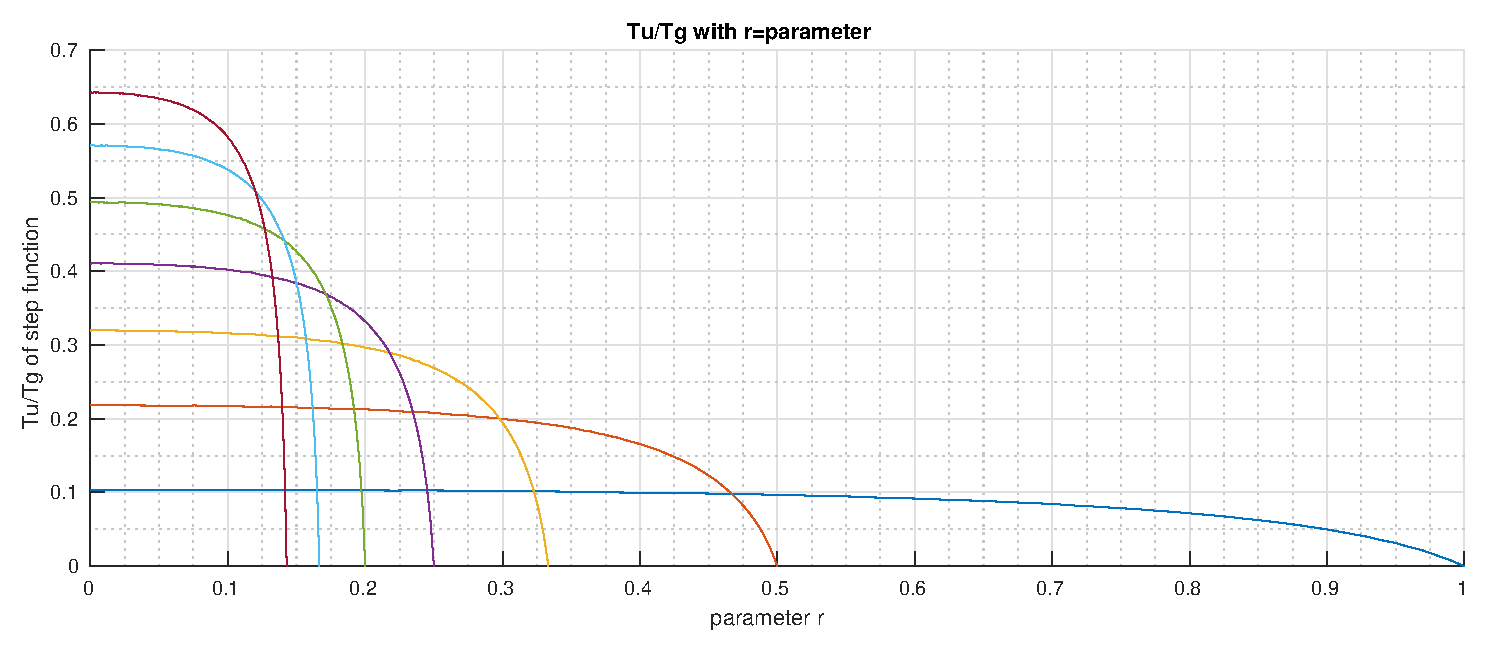
\includegraphics[width=\linewidth]{images/hudzovic_curves_tu_tg}
    \caption{Hudzovic Tu/Tg and 1/Tg lookup curves.}
    \label{fig:hudzovic_tu_tg}
\end{figure}
\begin{figure}
    \includegraphics[width=\linewidth]{images/sani_curves_tu_tg}
    \caption{Sani Tu/Tg and 1/Tg lookup curves.}
    \label{fig:sani_tu_tg}
\end{figure}
\begin{figure}
    \includegraphics[width=\linewidth]{images/hudzovic_curves_t10_t50_t90}
    \caption{Hudzovic (t90-t10/t50) and 1/t50 lookup curves.}
    \label{fig:hudzovic_t3}
\end{figure}
\begin{figure}
    \includegraphics[width=\linewidth]{images/sani_curves_t10_t50_t90}
    \caption{Sani (t90-t10)/t50 and 1/t50 lookup curves}
    \label{fig:sani_t3}
\end{figure}

Visualising   these   functions   yields    the    curves    seen    in   figure
\ref{fig:hudzovic_tu_tg}. What these plots show beautifully is  that  the higher
the order $n$, the steeper -- or more  ``complex''  -- the step response becomes
(smaller values of $T_g$ mean faster rise  times of the step responses). Another
important thing to observe is how lower orders of $G_n(s,r)$ aren't able to rise
as fast as higher orders are able to, \textbf{regardless} of $r$  and  $T$. This
can also be seen in figure \ref{fig:hudzovic_tu_tg},  lower  orders cannot reach
ratios of $T_u/T_g$ that higher orders can.

As discussed earlier, determining the complexity of a step  response is directly
related to the  required  order  $n$  of  the model. Finding $n$ is now a simple
matter  of  computing  $\textrm{plant}_{T_u/T_g}$  and  iterating   through  the
different  curves in figure \ref{fig:hudzovic_tu_tg} until we find an  $n$  that
satisfies the condition:

\begin{equation}
    g_{T_u/T_g}(r, n)\lvert_{r=0} \hspace{2mm} \le \hspace{2mm} plant_{T_u/T_g}
    \label{eq:find_n}
\end{equation}

Ideally,  we'd  like  $n$  to  be  as  small   as   possible,   hence   equation
\ref{eq:find_n}.

With the  parameter $n$ defined, the next step is to find the intersection point
of  $g_{T_u/T_g}(r, n)$ with the horizontal line  $plant_{T_u/T_g}$.  This  will
yield parameter $r$. This can be achieved by solving a simple  line intersection
equation  and  plugging  in  the   locations   of   the  two  horizontal  lines.

The last parameter, $T$, can finally be determined  by  evaluating $g_{1/T_g}(r,
n) \cdot T_g$. Graphically, this equates to finding the  intersection  point  of
the vertical line going through $r$ and the function $g_{1/T_g}(r, n)$ in figure
\ref{fig:hudzovic_tu_tg} and multiplying the result by $T_g$.


\subsection{Least Squares Fit}

Given a discrete set of data points which represent a measured step  response of
an  unknown system, the input parameters  of  the  function  $G_n(s,r)$  can  be
tweaked such that the squared error between its step response and the input data
is minimised. The squared error is computed using:

\begin{equation}
    S = \sum_{i} \left(g(t_i)-y_i\right)^2
\end{equation}

where $g(t)$ is the inverse Laplace transform  of $\frac{G_n(s,r)}{s}$ (the time
domain step response) and ($t_i$,$y_i$) are  data  points  of  the measured step
response.

By fitting a system $G_n(s,r)$ to  the  input  data,  it  is possible to further
refine the results  obtained by the two methods mentioned thus far, or otherwise
find  optimal  values  for  $T$  and  $r$ when dealing with  noisy  input  data.

The possibility of finding local minima exists. It is therefore advised to first
use one of the four previous methods to find optimal initial values for $T$, $r$
and $n$ before performing the fit.

It will be shown that the  least  squares  fit  approach  will  yield  the  most
accurate results by orders of magnitude. The downside to this method, of course,
is the large amount of computation time required.


